\documentclass[12pt, twoside]{article}
\documentclass[12pt, twoside]{article}
\usepackage[letterpaper, margin=1in, headsep=0.2in]{geometry}
\setlength{\headheight}{0.6in}
%\usepackage[english]{babel}
\usepackage[utf8]{inputenc}
\usepackage{microtype}
\usepackage{amsmath}
\usepackage{amssymb}
%\usepackage{amsfonts}
\usepackage{siunitx} %units in math. eg 20\milli\meter
\usepackage{yhmath} % for arcs, overparenth command
\usepackage{tikz} %graphics
\usetikzlibrary{quotes, angles}
\usepackage{graphicx} %consider setting \graphicspath{{images/}}
\usepackage{parskip} %no paragraph indent
\usepackage{enumitem}
\usepackage{multicol}
\usepackage{venndiagram}

\usepackage{fancyhdr}
\pagestyle{fancy}
\fancyhf{}
\renewcommand{\headrulewidth}{0pt} % disable the underline of the header
\raggedbottom
\hfuzz=2mm %suppresses overfull box warnings

\usepackage{hyperref}
\usepackage{float}

\title{Algebra 2}
\author{Chris Huson}
\date{November 2024}

\fancyhead[LE]{\thepage}
\fancyhead[RO]{\thepage \\ First and last name: \hspace{2.5cm} \,\\ Section: \hspace{2.5cm} \,}
\fancyhead[LO]{BECA / Huson / Precalculus: 3. Complex numbers \\* 11 December 2024}

\begin{document}

\subsubsection*{3.18 PreTest: Rational exponents and complex numbers \hfill A2.A.APR.6}
\begin{enumerate}[itemsep=0.5cm]
\subsubsection*{A2-APR.1 Perform operations with polynomials}
% Problem 1
\item Find the sum in standard form:
\[
(2x^2 - 3x - 5) + (x^2 - 6x + 9).
\] \vspace{4cm}

% Problem 2
\item Find the difference \(f(x) - g(x)\) as a polynomial in standard form, given:
\[
f(x) = 4x^4 - x^3 + 6x^2 - 2x + 3 \quad \text{and} \quad g(x) = x^4 + 3x^2 - 2x - 4.
\] \vspace{4cm}

\item Select each correct equation.
\begin{multicols}{2}
    \begin{enumerate}
    \item $x^2 - 16 = x^2 - 4^2$
    \item $x^2 - 16 = (x-4)(x+4)$
    \item $x^2 + 16 = (x-4)(x+4)$
    \item $x^2 - 8x + 16 = (x-4)^2$
    \item $x^2 + 8x + 16 = (x+4)^2$
    \item $x^2 - 8x - 16 = (x-4)^2$
    \end{enumerate}
\end{multicols}
        
\item Which equations represent correct polynomial identities?
\begin{multicols}{2}
    \begin{enumerate}
    \item \(x^3 + y^3 = (x + y)^3\)
    \item \(x^3 + y^3 = (x - y)(x^2 + xy + y^2)\)
    \item \(x^3 - y^3 = (x + y)(x^2 - xy + y^2)\)
    \item \(x^3 - y^3 = (x - y)(x^2 + xy + y^2)\)
\end{enumerate}
\end{multicols}
    
\newpage
\subsubsection*{A2-F.IF.7a Graph linear and quadratic functions, show key features}
\item One equation of a system is graphed. 
\begin{enumerate}
    \item Graph the second equation, labeling the intersections as ordered pairs.
    \item Find the value of the leading coefficient $a$ of the quadratic equation.
\end{enumerate}
\begin{multicols}{2}
    \hspace{1cm} $y = ax^2 + 3x - 7$ \\
    \columnbreak
    $3x - y = -3$
    \end{multicols}
     \vspace{3cm}

  \begin{center}
  \begin{tikzpicture}[scale=.635]
    \draw [help lines] (-10,-10) grid (10,10);
    \draw [thick, ->] (-10.2,0) -- (10.4,0) node [below right] {$x$};
    \draw [thick, ->] (0,-10.2)--(0,10.4) node [left] {$y$};
    \draw[thick, <->,smooth, domain=-3.3:2.1] plot (\x, {2.5*(\x)^2 + 3*\x - 7});
  \end{tikzpicture}
  \end{center}
  

\newpage
\subsubsection*{A2-A.APR.3 Identify zeros of polynomials given suitable factorizations}
\item Write down the solutions to the equation $x(x - 1)(2x + 5)(x + 4) = 0$. \vspace{2cm} 

\item The polynomial $p$ is a function of $x$. The graph of $p$ has three zeros at $-5$, $\frac{3}{2}$, and $-1$. Select $\bf{all}$ the expressions that could represent $p$. \vspace{0.25cm}
    \begin{multicols}{2}
    \begin{enumerate}
        \item $(x-5)(x-\frac{3}{2})(x+1)$
        \item $(x+5)(3x-2)(x+1)$
        \item $3(x+5)(x-\frac{3}{2})(x+1)$
        \item $3x(x+5)(x+\frac{2}{3})(x-1)^2$
        \item $(x-5)(x+\frac{2}{3})(x-1)$
        \item $(x+5)(2x-3)(x+1)$
        \item $3(x-5)(x-\frac{2}{3})(x-1)$
        \item $3x(x+5)(x-\frac{3}{2})(x+1)^2$
    \end{enumerate}
    \end{multicols}

\item Select the expression that is equivalent to $\displaystyle \frac{3x^2 + 10x - 8}{x - 2}$ for $x \neq 2$.
    \begin{enumerate}
        \item $\displaystyle 3x + 4 - \frac{16}{x - 2}$
        \item $\displaystyle 3x + 6 - \frac{10}{x - 2}$
        \item $\displaystyle 3x + 4 - \frac{8}{x - 2}$
        \item $\displaystyle 3x + 6 - \frac{14}{x - 2}$
    \end{enumerate}
    \vspace{3cm}
\newpage
 
\subsubsection*{A2-F.BF.2 Write arithmetic and geometric sequences with recursive formulas}
\item Write a recursive definition of the sequence $a_1 = -3$, $a_2 = 2$, $a_3 = 7$, $a_4 = 12, \ldots$ \vspace{2cm}

\item Write a recursive definition of the arithmetic sequence $b$. \\[0.5cm]
\renewcommand{\arraystretch}{1.5}
\begin{tabular}{|c|c|}
\hline
$n$ & $b_n$ \\
\hline
$1$ & $12$ \\
$2$ & $1.2$ \\
$3$ & $0.12$ \\
\hline
\end{tabular} \vspace{1cm}

\newpage 
\subsubsection*{A2-F.IF.7c Graph polynomials, identify zeros, end behavior}
\item Below is a graph of the polynomial $f(x)$. 
\begin{multicols}{2}
    \begin{enumerate}[itemsep=1cm]
        \item Is the leading coefficient positive or negative?
        \item Which of the following could be its equation?
    \begin{enumerate}
        \item $f(x)=(x+2)(x-4)(x-2)^2$
        \item $f(x)=(x-2)(x-4)(x+2)^2$
        \item $f(x)=(x+2)(x+4)(x-2)^2$
        \item $f(x)=(x-2)(x+4)(x+2)^2$
    \end{enumerate} \vspace{1cm} \;
    \end{enumerate}

    \columnbreak
    \begin{tikzpicture}[xscale=0.7, yscale=0.7]
        \draw[lightgray,very thin] (-5,-5) grid (4,4);
        \draw [thick, ->] (-5.2,0) -- (4.4,0) node [above] {$x$};
        \draw [thick, ->] (0,-5.2)--(0,4.5) node [right] {$y$};
        \foreach \x in {-5,4} \draw (\x cm,5pt) -- (\x cm,-5pt) node[below] {$\x$};
        \draw (5pt,4 cm) -- (-5pt,4 cm) node[left] {$40$};
        %\fill (-1,0) circle[radius=0.1] node[above left]{$j$};
        %\fill (3,0) circle[radius=0.1] node[above right]{$k$};
        \draw [thick, <->,smooth,samples=20,domain=-4.5:2.3] plot(\x,{0.1*(\x+4)*(\x-2)*(\x+2)^2});
    \end{tikzpicture}
\end{multicols}

\item The graph of the polynomial $f(x) = x^{4}-9x^{2}-4x+12$ is shown. 
    \begin{multicols}{2}
        \begin{enumerate}[itemsep=1cm]
            \item What is the degree of the function?
            \item What are the zeros of the function?
            \item Which factor has a multiplicity of 2?
            \item Write down the $y$-intercept as an ordered pair.
            \item Three points are marked on the graph, $p$, $q$, and $r$. Which one is a local minimum?
        \end{enumerate} \vspace{1cm} \;
    
        \columnbreak
    
        \begin{tikzpicture}[xscale=0.7, yscale=0.8]
            \draw[lightgray,very thin] (-4,-4) grid (4,5);
            \draw [thick, ->] (-4.2,0) -- (4.4,0) node [above] {$x$};
            \draw [thick, ->] (0,-4.2)--(0,5.5) node [right] {$y$};
            \foreach \x in {-4,4} \draw (\x cm,5pt) -- (\x cm,-5pt) node[below] {$\x$};
            \draw (5pt,5 cm) -- (-5pt,5 cm) node[left] {$20$};
            \draw [thick, <->,smooth,samples=20,domain=-3:3.3] plot(\x,{0.25*(\x-1)*(\x-3)*(\x+2)^2});
            \filldraw [black] (-0.27, 3.1) circle (2.5pt) node[above left]{$p$};
            \filldraw [black] (1, 0) circle (2.5pt) node[above right]{$q$};
            \filldraw [black] (2.23, -4.2) circle (2.5pt) node[above]{$r$};
        \end{tikzpicture}
    \end{multicols}

\newpage
\item The graph of the function $f(x) = x^3 - 3x^2 - 10x + 24$ is shown. Write the function in factored form. 
    \begin{flushright}
    \begin{tikzpicture}[xscale=1, yscale=0.25]
        \draw [thick, ->] (-4.2,0) -- (5,0) node [above] {$x$};
        \draw [thick, ->] (0,-8.2)--(0,10) node [right] {$y$};
        \foreach \x in {-3,...,4} \draw (\x cm,12pt) -- (\x cm,-12pt) node[below] {$\x$};
        %\foreach \y in {-8,-6,4,8} \draw (3pt,\y cm) -- (-3pt,\y cm) node[left] {$\y$};
        \draw [thick, <->,smooth,samples=20,domain=-3.6:4.6] plot(\x,{0.3*(\x-2)*(\x-4)*(\x+3)});
    \end{tikzpicture}
    \end{flushright}

\item Let $j(x)= (x+4)(x+1)(x-4)^2$ be a polynomial function. 
    \begin{center}
    \begin{tikzpicture}[xscale=0.7, yscale=0.7]
        \draw [thick, ->] (-7.2,0) -- (7.5,0) node [above] {$x$};
        \draw [thick, ->] (0,-5.2)--(0,6.5) node [right] {$y$};
        \foreach \x in {-7,...,7} \draw (\x cm,5pt) -- (\x cm,-5pt);
    \end{tikzpicture}
    \end{center}
    \begin{enumerate}[itemsep=0.25cm]
        \item Sketch a graph of the function. Label the $x$-intercepts.
        \item Find the value of the $y$-intercept and mark it on the graph. \vspace{1cm}
        \item Identify the end behavior of the function.
            \begin{multicols}{2}
            \begin{enumerate}
                \item As $x \to +\infty$, $y \to +\infty$; \\ 
                as $x \to -\infty$, $y \to -\infty$
                \item As $x \to +\infty$, $y \to -\infty$; \\
                as $x \to -\infty$, $y \to +\infty$
                \item As $x \to +\infty$, $y \to +\infty$; \\
                as $x \to -\infty$, $y \to +\infty$
                \item As $x \to +\infty$, $y \to -\infty$; \\
                as $x \to -\infty$, $y \to -\infty$        
            \end{enumerate}
            \end{multicols}
    \end{enumerate}

\newpage

\subsubsection*{HSN.RN.2 Expressions with radicals and rational exponents}
\item Simplify each radical expression.
    \begin{multicols}{2}
    \begin{enumerate}[itemsep=0.5cm]
        \item $\sqrt{49}=$
        \item $\sqrt{32}=$
        \item $\sqrt{-45}=$
        \item $\displaystyle \frac{\sqrt{-12}}{\sqrt{3}}=$
    \end{enumerate}
    \end{multicols} \vspace{1cm}
    
\item Simplify each expression.
    \begin{multicols}{2}
    \begin{enumerate}[itemsep=0.5cm]
        \item $\displaystyle 8^{\frac{2}{3}} =$
        \item $\left( \sqrt{\frac{4}{9}} \right)^{3} =$
    \end{enumerate}
    \end{multicols} \vspace{2cm}

    
\item Rewrite each expression as a fractional exponent in simplest terms.
    \begin{multicols}{2}
      \begin{enumerate}[itemsep=1cm]
          \item $\sqrt[3]{3} =$
          \item $\displaystyle \frac{1}{\sqrt[2]{3}}=$
          \item $\sqrt[4]{x^3} =$
          \item $\displaystyle \frac{1}{(\sqrt[4]{x})^2}=$
      \end{enumerate}
      \end{multicols} \vspace{1cm}
  
\item Rewrite each expression with fractional exponent as a radical.
    \begin{multicols}{2}
      \begin{enumerate}[itemsep=1cm]
        \item $\displaystyle 3^{\frac{1}{2}}=$
        \item $\displaystyle 3^{-\frac{2}{3}}=$
        \item $\displaystyle x^{\frac{1}{3}}=$
        \item $\displaystyle x^{-\frac{2}{3}}=$
      \end{enumerate}
      \end{multicols}

\subsubsection*{A2-A.SSE.3c Apply the properties of exponents}
\item Identify the expressions that are equal to $\displaystyle \frac{3^3}{3^5}$
    \begin{multicols}{2}
    \begin{enumerate}
        \item $3^{-2}$
        \item $\frac{1}{9}$
        \item $3^{3}$
        \item $3^8$
        \item $\displaystyle \frac{1}{3^2}$        
        \item $0.111$
    \end{enumerate}
    \end{multicols}

\item Identify the expressions that are equal to $\displaystyle 5^{-2}$
    \begin{multicols}{2}
    \begin{enumerate}
        \item $\displaystyle \frac{1}{5^2}$
        \item $5.5$
        \item $\sqrt{5}$        
        \item $\displaystyle \frac{1}{25}$
        \item $0.04$        
        \item $10$
    \end{enumerate}
    \end{multicols}

\item Identify the expressions that are equal to $\displaystyle 16^{\frac{1}{4}}$
    \begin{multicols}{2}
    \begin{enumerate}
        \item $2$        
        \item $4$        
        \item $\sqrt{4}$
        \item $\sqrt[4]{16}$
        \item $16.25$
        \item $256$
    \end{enumerate}
    \end{multicols}
        
\newpage
\subsubsection*{6.EE.b Reason about and solve one-variable equations and inequalities}
% (A.REI.4 Solve quadratic equations algebraically)

\item Use the function $f(x) = \frac{1}{2}x + 11$ to answer the questions.
    \begin{multicols}{2}
    \begin{enumerate}[itemsep=2cm]
        \item Find the value of $f(4)$.
        \item Solve for $x$ if $f(x) = 2$.
    \end{enumerate}
    \end{multicols} \vspace{2cm}

    
\item Solve each equation for $x$.
\begin{multicols}{2}
    \begin{enumerate}
    \item $x^2+5x+6 = 0$
    \item $x^3-7x^2+6x = 0$ 
    \end{enumerate} 
\end{multicols} \vspace{3cm}

\item The expression $\displaystyle 2 - \frac{x - 1}{x + 2}$ is equivalent to 
\begin{multicols}{2}
    \begin{enumerate}
    \item $\displaystyle 1 - \frac{3}{x + 2}$
    \item $\displaystyle 1 + \frac{3}{x + 2}$ 
    \item $\displaystyle 1 - \frac{1}{x + 2}$
    \item $\displaystyle 1 + \frac{1}{x + 2}$ 
    \end{enumerate} 
\end{multicols} 

\item Find all of the values of $x$ that make the equation true. 
$$\frac{3}{x-4} = \frac{x-5}{x}$$ \vspace{4cm}

\newpage
      
\item Given the rational function $\displaystyle r(x)= 3 -\frac{x - 1}{x + 2}$. % F.IF.7d Graph rational functions
        \begin{enumerate}[itemsep=0.25cm]
            \item Sketch a graph of the function.
            \item Mark the vertical asymptote as dotted line and label it with its equation.
            \item Explain why the asymptote is located there.
        \end{enumerate}
        \begin{center}
        \begin{tikzpicture}[xscale=0.7, yscale=0.7]
            \draw [thick, ->] (-10.2,0) -- (10.5,0) node [above] {$x$};
            \draw [thick, ->] (0,-10.2)--(0,10.5) node [right] {$y$};
            \foreach \x in {-10,-8,-6,-4,-2,2,4,6,8,10} \draw (\x cm,5pt)--(\x cm,-5pt) node at (\x,-0.5){\x};
            \foreach \y in {-10,-8,-6,-4,-2,2,4,6,8,10} \draw (5pt,\y cm)--(-5pt,\y cm) node at (-0.5,\y){\y};
        \end{tikzpicture}
        \end{center}



\end{enumerate}
\end{document}